\documentclass{article}
\pagestyle{plain}

\author{Ramyad Hadidi}
\date{\today}

\usepackage{graphicx}
\usepackage{amsmath}
\usepackage{listings}
\usepackage{color}
\usepackage{hyperref}
\usepackage[usenames,dvipsnames]{xcolor}


\begin{document}

\definecolor{light-blue}{RGB}{216,208,255}
\lstset{language=C++, 
	basicstyle=\fontsize{9}{9}\selectfont\ttfamily,
        keywordstyle=\color{Blue}\ttfamily,
        stringstyle=\color{Red}\ttfamily,
        commentstyle=\color{ForestGreen}\ttfamily,
        breaklines=true
	backgroundcolor=\color{light-blue}, 
	frame=single,
	numbers=left, 
	stepnumber=1,
	numberstyle=\tiny\color{Sepia},
	morekeywords={}}

	
\begin{minipage}[t]{1.0\textwidth}
 \emph{\indent\textbf{Report:} \\
		   \-\ Memory Coalescing for GPUs \\
		   \-\ Assignment 5 GPU Architecture Course \\
		   \-\ Ramyad Hadidi - \today
  }
\end{minipage}

\vspace{3 mm}
\hrule
\vspace{3 mm}

\section{Introduction}
In this assignment, trace generation is implemented in previously developed Harmonica ISA emulator \footnote{\url{https://github.com/ramyadhadidi/harmonica_emulator_proj}}. Also, in emulator different mechanisms for memory coalescing is integrated. Therefore, with the help of the emulator a study on memory coalescing effects on cache has been done using Dinero IV\footnote{\url{http://pages.cs.wisc.edu/~markhill/DineroIV/}} a Trace-Driven Uniprocessor Cache Simulator. In this report first we show how memory coalescing code was integrated, then a study about impact of cache line size on cache performance, and finally another study about memory mapping schemes and its impact on cache performance.

The benchmarks that we are using is \emph{small} version of \emph{vecsum} and \emph{scan} applications with 8 threads/warp and 32 threads/warp\footnote{16 threads/warp was not supplied for small version of traces}. For Dinero, we use one level cache with fixed properties except of cache line size in the first study. We have used a 32KB, 4 way set-associative cache with 8 banks.

\section{Developed Code}
In each execution step, the main class of \emph{core\_c} will call \emph{step()} function, which it will call all warp in the core and execute them. In each warp after executing all threads, if threads encounter ST or LD, they will save their address to variable \emph{m\_coalMemAddr} and the number of them in \emph{m\_uniqeCoalMemAddr}. At the end of the execution of a warp, a \emph{coalesce()} function will be called and address will be coalesced based on global configurations, such as cache line size and mapping scheme. Here is the code:
\begin{lstlisting}
void warp_c::coalesce() {
  unsigned maximumDistance = (1LL << CACHE_LINE_IN_BYTE/WORD_SIZE_IN_BYTE) - 1;
  set<Addr> memAddresses;
  set<Addr> coalMemAddr;

  //Get inputs
  for (unsigned int i=0; i<m_uniqeCoalMemAddr ; i++)
    memAddresses.insert( m_coalMemAddr[i] );

  //Note: set will not insert duplicate element
  for (set<Addr>::iterator itA = memAddresses.begin(); itA != memAddresses.end();) {
    bool coalFound = false;
    for (set<Addr>::iterator itB = memAddresses.begin(); itB != memAddresses.end();) {
      Addr firstElem = *itA >> RIGHT_BIT_SHIFT_COAL;
      Addr secondElem = *itB >> RIGHT_BIT_SHIFT_COAL;
      Addr mask = (1LL << RIGHT_BIT_SHIFT_COAL) - 1;
      Addr lowerFirstElem = *itA & mask;
      Addr lowerSecondElem = *itB & mask;
      if ( (abs(secondElem - firstElem) < maximumDistance) && (*itB != *itA) && (lowerFirstElem == lowerSecondElem) ) {
        coalFound = true;
        memAddresses.erase(itB++);
        coalMemAddr.insert(*itA);
      }
      else {
        itB++;
		m_core->statNotCoalesced ++;
      }
    }
    //Uniqe item itslef, insert it
    if (!coalFound)
      coalMemAddr.insert(*itA);
    memAddresses.erase(itA++);
  }

  //Restore outputs
  int sizeOld = m_uniqeCoalMemAddr;
  m_uniqeCoalMemAddr = coalMemAddr.size();
  unsigned int i=0;
  for (set<Addr>::iterator it = coalMemAddr.begin(); it != coalMemAddr.end(); ++it, ++i) 
    m_coalMemAddr[i] = *it;
  m_core->statCoalesced += sizeOld-m_uniqeCoalMemAddr;
}
\end{lstlisting}
First, the elements of m\_coalMemAddr have been copied to a set. Set is used because it will not allow duplicate elements. Also, set will order the addresses which enable us to write a 2 for loop for coalescing and select the first item as the representative cache line if coalescing criteria passed. In the 2 for loop body we check if the 2 addresses has coalescing ability based on maximum distance (based on cache line size) and also if coalescing is based on higher value bits we check equality of lower bits.
In addition I have used a statistics to show how many coalescing is occurring versus not coalesced accesses.

\section{Cache Line Size Study}
In this study coalescing based on lower bits is done and the impact of changing cache line size on different cache performance metrics has been studied. In figure \ref{cachelinesize} miss rate is shown for different warp size and cache line size. As we can see in all cases miss rate is decreasing. Also, an interesting point is between 8 warp and 32 warp version which shows 32 warp size is getting more benefit from cache line size 64 to 128 than 8 warp size. This is because 32 warp accesses has more covering. Figure \ref{demandfetches} shows reduction in demand fetches and therefore pressure on memory system.

\begin{figure}[h!]
  \centering
  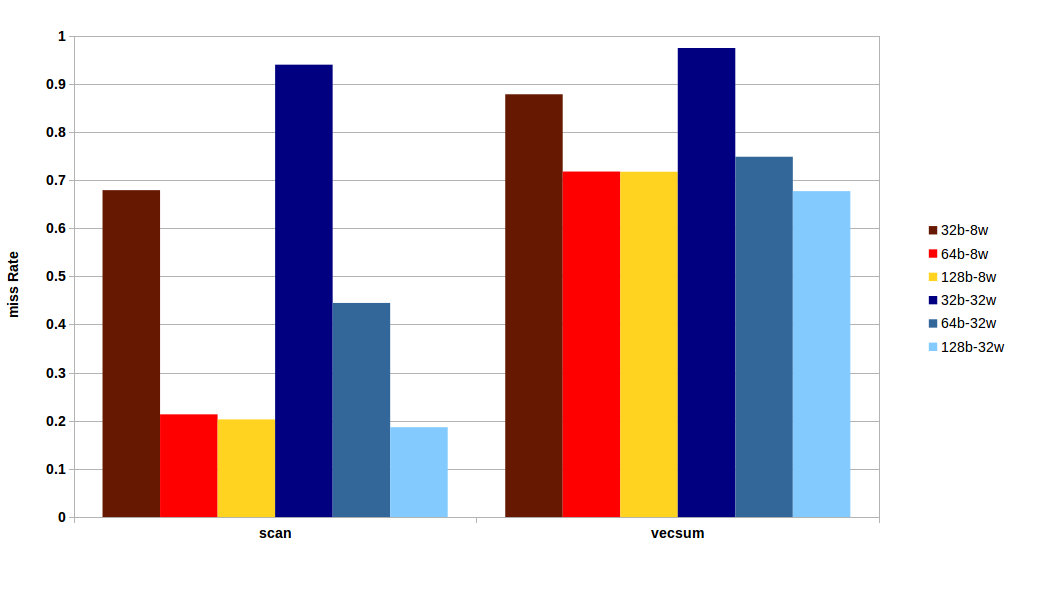
\includegraphics[width=1.0\textwidth]{cachelinesize_1.png}
  \caption{Miss Rate with Different Cache Line Size}
  \label{cachelinesize}
\end{figure}

\begin{figure}[h!]
  \centering
  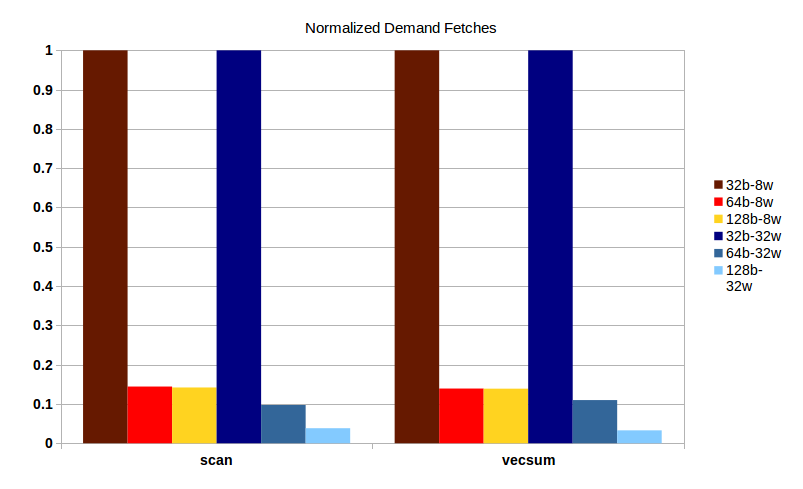
\includegraphics[width=1.0\textwidth]{demandfetches.png}
  \caption{Normalized Demand Fetches}
  \label{demandfetches}
\end{figure}

\clearpage

\section{Mapping Scheme}
For this section cache line size is 32 Bytes. The schemes are different in which bits they choose for coalescing. The main metric I use to select coalescing on which bits are more beneficial for an applications is the number of coalesced request versus number of non coalesced request. After a study on different bits for coalescing, for both applications I found mapping based on \textbf{bits 19~12} gives the most coalesced accesses. In figure \ref{bitsgraph} I have shown the cache performance metrics with the base line of coalescing with lower bits and no coalescing. Basic Coalescing miss rate is higher since it just reduces number of demand fetches but the ratio stays the same.

\begin{figure}[h!]
  \centering
  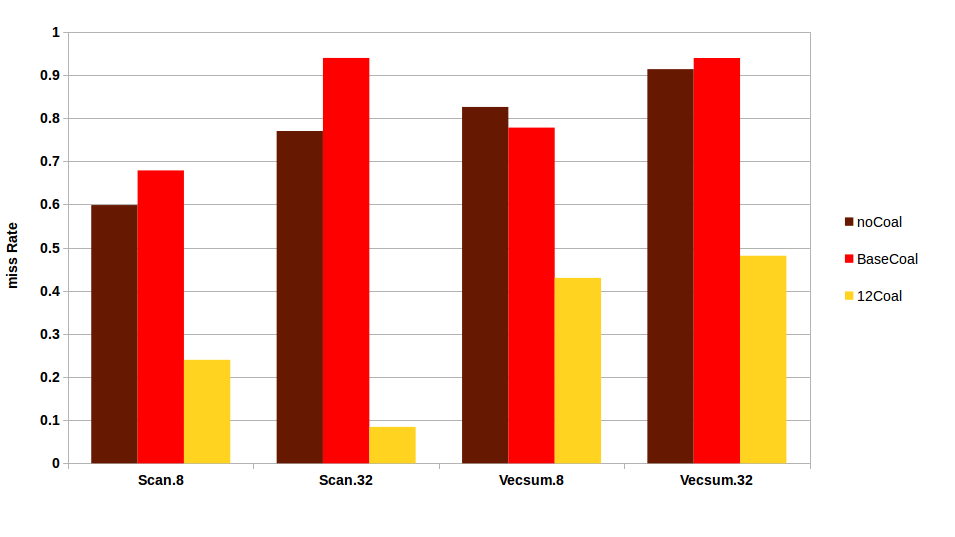
\includegraphics[width=1.0\textwidth]{bitsgraph.png}
  \caption{Mapping Schemes Miss Rates}
  \label{bitsgraph}
\end{figure}

%\bibliographystyle{plain}
%\bibliography{refrences}
\end{document}